\documentclass{article}

\usepackage[preprint]{neurips_2024}

\usepackage[utf8]{inputenc}
\usepackage[T1]{fontenc}
\usepackage{hyperref}
\usepackage{url}
\usepackage{booktabs}
\usepackage{graphicx}
\usepackage{amsmath}
\usepackage{microtype}
\usepackage{xcolor}

\title{Language-Conditioned Basket Sorting with a Panda Arm in MuJoCo}

\author{%
  Hui Xu\\
  ESE 577 Final Project\\
  \texttt{huixu3}\\
}

\begin{document}

\maketitle

\begin{abstract}
This project implements a language-conditioned pick-and-place system for a Franka Panda-style robot arm in MuJoCo. The task is to place one of two YCB objects, a red cracker box or a yellow mustard bottle, into one of two colored baskets according to a natural-language command supplied at run time. The final system combines a lightweight language parser, a finite-state pick-and-place policy, a continuity-aware differential inverse kinematics controller, and a MuJoCo scene built from course Panda assets and public YCB meshes. The scripted model-based executor solved all 300 randomized evaluation episodes in the class Panda scene, with an average of 90.84 control steps per episode. A five-task video artifact is included in the submission and shows variability across object, basket, and speed instructions.
\end{abstract}

\section{Introduction}

Language-conditioned manipulation is useful because it separates the user's goal from the robot's low-level control interface. Instead of directly specifying joint targets, the user can say ``place the mustard bottle in the right basket'' and the robot must infer both the target object and the target location. This project focuses on a compact version of that problem: sorting two tabletop objects into two baskets using a Panda arm.

The original project proposal considered an end-effector waypoint pipeline followed by inverse kinematics and control. A concern with that approach is that independently solving inverse kinematics for consecutive end-effector targets can produce discontinuous joint-space motions, for example switching between elbow-up and elbow-down solutions for nearby Cartesian poses. To avoid that failure mode, the final implementation uses differential inverse kinematics seeded by the current joint state. Each step computes a small joint update from the local Jacobian, clips large joint jumps, and respects joint limits. This keeps consecutive actions compatible with each other while preserving a simple Cartesian policy interface.

The final system is intentionally pragmatic. The policy used for final evaluation is a model-based finite-state machine (FSM), not a learned vision-language policy. I also implemented demonstration collection and a simple behavior cloning baseline to keep a learning path available, but the learned baseline was not strong enough to use as the final executor. The FSM provides a reliable final product for the assignment: it can be installed with a few Python dependencies, run from the command line, and repeatedly solve randomized versions of the manipulation task.

\section{Task and assets}

The task scene contains a Panda arm, two movable objects, and two baskets. The class Panda scene is located at \path{assets/class_panda/basket_scene.mjcf}. It uses the homework Panda MJCF and mesh assets extracted from the course homework zip, plus public YCB Google 16k meshes for the cracker box and mustard bottle. The color convention used in the final demo is shown in Table~\ref{tab:scene}.

\begin{table}[h]
\centering
\caption{Objects and baskets in the final MuJoCo scene.}
\label{tab:scene}
\begin{tabular}{lll}
\toprule
Entity & Visual color & Semantic label \\
\midrule
YCB cracker box & Red & \texttt{cracker\_box} \\
YCB mustard bottle & Yellow & \texttt{mustard\_bottle} \\
Left basket & Blue & \texttt{left} basket \\
Right basket & Green & \texttt{right} basket \\
\bottomrule
\end{tabular}
\end{table}

Although the cleanest demo convention is red/cracker to blue/left and yellow/mustard to green/right, evaluation is not hard-coded to that mapping. The environment samples language commands that may request either object and either basket. This tests whether the decision pipeline follows the command rather than memorizing a fixed visual color rule.

\section{Method}

\subsection{System overview}

The robot decision-making pipeline has four main components:

\begin{enumerate}
  \item A language parser extracts the target object, target basket, and speed modifier from the instruction.
  \item A scripted FSM converts the parsed task into a sequence of end-effector goals: approach, descend, grasp, lift, move above the basket, lower, release, and retreat.
  \item A differential IK controller converts each Cartesian target into a continuous joint-space update.
  \item The MuJoCo environment applies the arm and gripper commands, updates object attachment during grasps, and checks success.
\end{enumerate}

All policies use the same action interface:
\[
  a_t = [x_t, y_t, z_t, g_t],
\]
where $(x_t, y_t, z_t)$ is the desired end-effector target and $g_t$ is the gripper command. Positive gripper values mean open, and negative values mean close. This interface lets the same FSM and behavior-cloning code run in both the lightweight kinematic fallback environment and the MuJoCo class scene.

\subsection{Language parsing}

The parser is rule-based because the command grammar is intentionally small. It detects object words such as ``cracker,'' ``box,'' ``mustard,'' and ``bottle,'' basket words such as ``left'' and ``right,'' and optional speed words such as ``careful'' or ``fast.'' The parsed task is stored as a structured task specification. This is enough for the current task distribution, and it makes evaluation deterministic and easy to debug.

At run time, the user can provide the language instruction directly through the command-line interface. For example, the following command makes the robot repeatedly execute the requested red/cracker to blue/left task under randomized object starts:

\begin{center}
\path{python scripts/evaluate.py --config configs/class_panda.yaml --policy fsm --instruction "place the cracker box in the left basket" --episodes 3}
\end{center}

Changing only the instruction string changes the selected object and basket:

\begin{center}
\path{python scripts/evaluate.py --config configs/class_panda.yaml --policy fsm --instruction "place the mustard bottle in the right basket" --episodes 3}
\end{center}

To make this visible in the submitted artifacts, the video writer overlays the executed command on every saved GIF frame with a caption beginning with ``Language:''. The evaluation JSON also stores the same string in each episode's \texttt{instruction} field. This means the video itself shows which language command was entered, while the log file provides a machine-readable record of the same command.

\subsection{Finite-state pick-and-place policy}

The FSM policy is implemented in \path{src/basket_sorting/fsm.py}. Given the current observation, it computes a target waypoint for the active phase. The phases are:

\begin{center}
\texttt{approach} $\rightarrow$ \texttt{descend} $\rightarrow$ \texttt{grasp} $\rightarrow$ \texttt{lift} $\rightarrow$ \texttt{move\_to\_basket} $\rightarrow$ \texttt{lower} $\rightarrow$ \texttt{release} $\rightarrow$ \texttt{retreat}.
\end{center}

The FSM switches phases when the end-effector is close enough to the current waypoint or after the gripper command has been held for enough steps. Speed words modify the commanded motion step size; for example, ``careful'' moves more slowly than ``fast.'' The FSM is model-based and uses object positions from the MuJoCo state, so it is best understood as a reliable expert controller rather than a perception-based learned policy.

\subsection{Differential inverse kinematics}

The controller avoids solving each IK target independently. At time $t$, it computes the end-effector position $p(q_t)$ and Jacobian $J(q_t)$ at the current joint configuration. For a desired Cartesian displacement $\Delta x$, it solves a damped least-squares update:
\[
  \Delta q = J^\top (JJ^\top + \lambda^2 I)^{-1} \Delta x.
\]
The update is then clipped by a maximum joint-step threshold and by joint limits. This makes the local IK solution continuous from the previous state and reduces the risk of sudden joint discontinuities. The same controller interface is used with a toy kinematic backend for the fallback environment and a MuJoCo Jacobian backend for the class Panda scene.

\subsection{Grasp and object handling}

The MuJoCo environment contains free joints for the two YCB objects. During evaluation, a grasp is detected when the gripper is closed near the target object at the configured grasp height. Once attached, the object pose is updated relative to the end-effector until the gripper opens over the basket. This creates a stable manipulation benchmark for testing language-conditioned decision making and IK continuity without requiring a full contact-rich grasp controller.

\subsection{Learning baseline}

The repository also includes scripts for collecting FSM demonstrations and fitting a lightweight behavior cloning baseline. Demonstrations store state features, subtask text, speed, and the low-level action. The current NumPy linear behavior cloning model is included as a smoke-test baseline only. In previous testing on the class scene it achieved 0/20 successes, while the FSM achieved 20/20. Because the assignment asks for a final product that reliably solves the task, the FSM is used as the final executor.

\section{Results}

\subsection{Evaluation protocol}

The main evaluation used \path{configs/class_panda.yaml}. Each episode samples a random target object, target basket, speed word, and initial object placement. Success is counted when the commanded target object is released inside the commanded basket. The final 300-episode evaluation was run with:

\begin{center}
\path{python scripts/evaluate.py --config configs/class_panda.yaml --policy fsm --episodes 300}
\end{center}

The required five-task video was generated with:

\begin{center}
\path{python scripts/evaluate.py --config configs/class_panda.yaml --policy fsm --episodes 5 --save-video videos/class_panda_fsm_eval_5.gif --video-episodes 5}
\end{center}

\subsection{Quantitative results}

Table~\ref{tab:results} reports the final quantitative results. The 300-episode run includes all four object-basket combinations. The sampled commands were balanced enough to test both objects and both baskets: 158 mustard episodes, 142 cracker episodes, 139 right-basket episodes, and 161 left-basket episodes.

\begin{table}[h]
\centering
\caption{Final FSM evaluation results in the class Panda MuJoCo scene.}
\label{tab:results}
\begin{tabular}{lrrrrr}
\toprule
Evaluation & Episodes & Successes & Success rate & Avg. steps & Step range \\
\midrule
Five-task video run & 5 & 5 & 100\% & 87.60 & 73--103 \\
Explicit cracker-to-left command & 3 & 3 & 100\% & 84.00 & 83--85 \\
Explicit mustard-to-right command & 3 & 3 & 100\% & 86.33 & 73--94 \\
Main evaluation & 300 & 300 & 100\% & 90.84 & 73--113 \\
\bottomrule
\end{tabular}
\end{table}

\subsection{Qualitative results}

Figure~\ref{fig:snapshots} shows snapshots from the generated five-task video. The sequence illustrates the robot observing two objects, closing the gripper on the target object, carrying it over a basket, and releasing it. The full video file is included at \path{videos/class_panda_fsm_eval_5.gif}.

I also include two instruction-specific videos to make the language interface explicit: \path{videos/language_red_to_blue.gif} was generated from ``place the cracker box in the left basket,'' and \path{videos/language_yellow_to_green.gif} was generated from ``place the mustard bottle in the right basket.'' In both cases, the GIF frames contain the command as an on-screen language caption, the printed evaluation logs show the same instruction string for each episode, and the robot acts on that specified object-basket pair. Since most PDF viewers do not reliably play animated GIFs, the report includes still frames from these GIFs in Figure~\ref{fig:language_demos}, while the submission zip includes the full animated GIF files.

\begin{figure}[h]
\centering
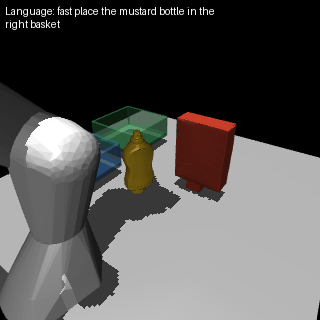
\includegraphics[width=0.19\linewidth]{figures/task_snapshot_0000.png}
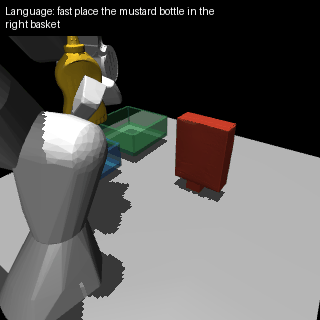
\includegraphics[width=0.19\linewidth]{figures/task_snapshot_0060.png}
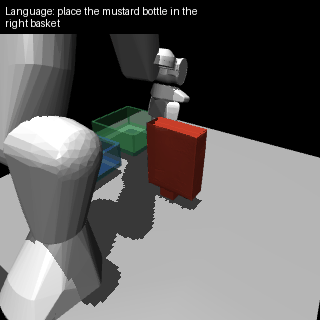
\includegraphics[width=0.19\linewidth]{figures/task_snapshot_0120.png}
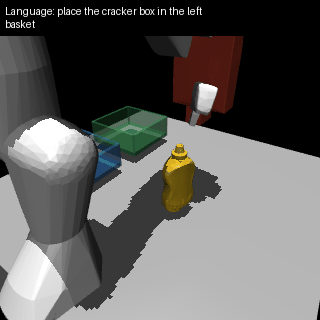
\includegraphics[width=0.19\linewidth]{figures/task_snapshot_0220.png}
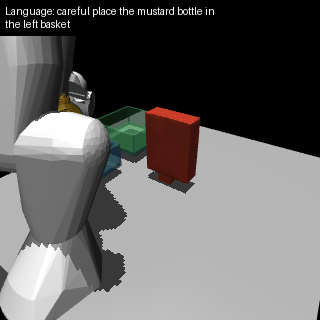
\includegraphics[width=0.19\linewidth]{figures/task_snapshot_0437.png}
\caption{Snapshots from the five-task MuJoCo video artifact. The camera view was chosen so that the red cracker box, yellow mustard bottle, blue left basket, green right basket, and Panda gripper are visible.}
\label{fig:snapshots}
\end{figure}

\begin{figure}[h]
\centering
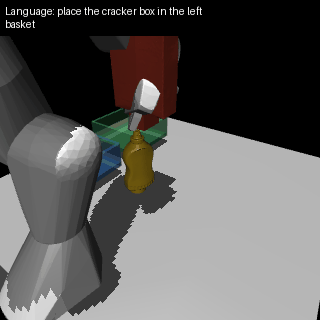
\includegraphics[width=0.46\linewidth]{figures/language_red_to_blue_snapshot.png}
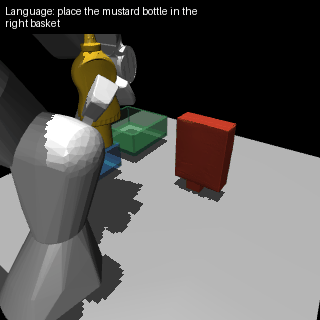
\includegraphics[width=0.46\linewidth]{figures/language_yellow_to_green_snapshot.png}
\caption{Still frames from the two explicit language-command GIFs. The caption at the top of each frame is the command provided through the command-line interface, making the language input visible in the report PDF as well as in the video artifacts.}
\label{fig:language_demos}
\end{figure}

\subsection{Discussion and limitations}

The main result is that the model-based executor is reliable on the target task distribution. The use of differential IK made the Cartesian waypoint policy smooth enough for repeated randomized trials, and the language parser was sufficient for the command set used in this project.

The main limitation is that the final policy uses privileged object poses from simulation. It does not yet estimate object poses from RGB images. The behavior cloning baseline also remains weak because the simple linear policy does not capture the phase-dependent structure of the task. A stronger learned version would use an image encoder, language embeddings, and a recurrent or transformer policy, while retaining the current differential IK controller as a low-level action interface. Another limitation is that grasping is represented with an attachment rule rather than full contact-rich manipulation. This keeps the benchmark stable but does not test all failure modes of a physical gripper.

\section{Code and reproducibility}

The repository includes a README with installation and run instructions. The shortest setup path is:

\begin{center}
\path{python -m venv .venv}

\path{.\.venv\Scripts\python.exe -m pip install -e ".[mujoco]"}

\path{.\.venv\Scripts\python.exe scripts/evaluate.py --config configs/class_panda.yaml --policy fsm --episodes 5 --save-video videos/class_panda_fsm_eval_5.gif --video-episodes 5}

\path{.\.venv\Scripts\python.exe scripts/evaluate.py --config configs/class_panda.yaml --policy fsm --instruction "place the mustard bottle in the right basket" --episodes 3 --save-video videos/language_yellow_to_green.gif}
\end{center}

The most important files are:

\begin{itemize}
  \item \path{README.md}: installation and evaluation instructions.
  \item \path{configs/class_panda.yaml}: final class Panda scene configuration.
  \item \path{assets/class_panda/basket_scene.mjcf}: MuJoCo scene with Panda, YCB objects, baskets, and demo camera.
  \item \path{src/basket_sorting/fsm.py}: scripted decision policy.
  \item \path{src/basket_sorting/envs/mujoco_env.py}: MuJoCo environment and differential IK integration.
  \item \path{scripts/evaluate.py}: evaluation entry point.
\end{itemize}

\section{References}

\begin{thebibliography}{9}

\bibitem{todorov2012mujoco}
Emanuel Todorov, Tom Erez, and Yuval Tassa.
\newblock MuJoCo: A physics engine for model-based control.
\newblock In \emph{IEEE/RSJ International Conference on Intelligent Robots and Systems}, 2012.

\bibitem{calli2015ycb}
Berk Calli, Arjun Singh, Aaron Walsman, Siddhartha Srinivasa, Pieter Abbeel, and Aaron M. Dollar.
\newblock The YCB object and model set: Towards common benchmarks for manipulation research.
\newblock In \emph{International Conference on Advanced Robotics}, 2015.

\bibitem{siciliano2010robotics}
Bruno Siciliano, Lorenzo Sciavicco, Luigi Villani, and Giuseppe Oriolo.
\newblock \emph{Robotics: Modelling, Planning and Control}.
\newblock Springer, 2010.

\bibitem{panda}
Franka Emika.
\newblock Panda robot documentation and model resources.
\newblock \url{https://franka.de/}.

\bibitem{mujocomenagerie}
Google DeepMind.
\newblock MuJoCo Menagerie robot model collection.
\newblock \url{https://github.com/google-deepmind/mujoco_menagerie}.

\end{thebibliography}

\end{document}
